\documentclass{article}
\usepackage{graphicx} % for figures
\usepackage{cite} % for citation
\usepackage{amsmath} % for piecewise function

\title{An Adaptive Hyperdynamics Method (AHDM) algorithm for Global Hyperdyanmics (GHD) Simulations}
\author{Jianming Cui}

\begin{document}
\bibliographystyle{unsrt}
\maketitle

Hyperdynamics (HD) is a method for accelerating the standard molecular dynamics (MD). It can significantly accelerate the simulations with rare events by adding an interatomic potential boost. In this report, we introduce an adaptive hyperdynamics method (AHDM) algorithm for global hyperdynamics (GHD). In GHD simulations, we have to decide how big the potential boost is and the best boosts are usually different in different cases. The AHDM algorithm will decide a best boost for a certain event.

\section{Preparation to run GHD}

\subsection{Parameters}

To run GHD, we need to set up the following parameters: temperature (T), the maxmimum bond boost ($V_{max}$), the boost threshold (q) which determine the max strain at which the bias potential goes to zero, the cutbond ($D_{bond}$) and the event threshold ($D_{event}$). Plimpton\cite{Plimpton2020} summarized some principles to set up the parameters. q is usually setted up as 0.3 for a distance less than the distance that an atom in a biased bond would displace from a quenched position to the nearest dividing surface for an adjacent energy basin. $D_{bond}$ should be 15\% bigger than the nearest-neighbor distance. $D_{event}$ should be some large fraction of the nearest neighbor.

\subsection{Simulation system and software}

We simulate the event that a single Ag atom diffuses on Ag(100), as shown in Figure 1. We decide to work on GHD first because there are less parameters and GHD is good enough to accelerate the simulations for small systems. 

The software we use is LAMMPS, version 03Mar2020, compiling with 'REPLICA', 'MANYBODY' and 'MOLECULE' packages. The 'REPLICA' package is required for running HD simulations. The 'MANYBODY' and the 'MOLECULE' packages are for the atom styles in this Ag system.

\begin{figure}[ht]
	\centering
  	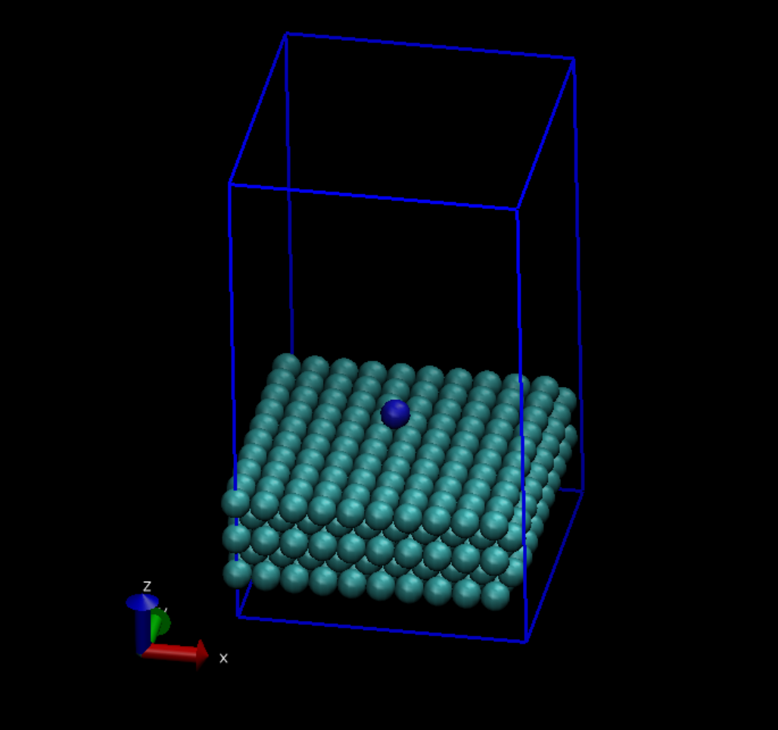
\includegraphics[height=4cm]{system.png}
  	\caption{Single Ag diffusion on Ag(100). The plane size is 10*10*5, shown in cyan. The blue ball is the Ag adatom that diffuses. The blue lines constitute the periodic boundary.}
\end{figure}

In this case, we use 0.3 for q, 3.32{\AA} for $D_{bond}$ (NN distance of Ag is 2.89{\AA}) and 1.2{\AA} for $D_{event}$.

\section{What is the best boost}

\begin{figure}[ht]
	\centering
  	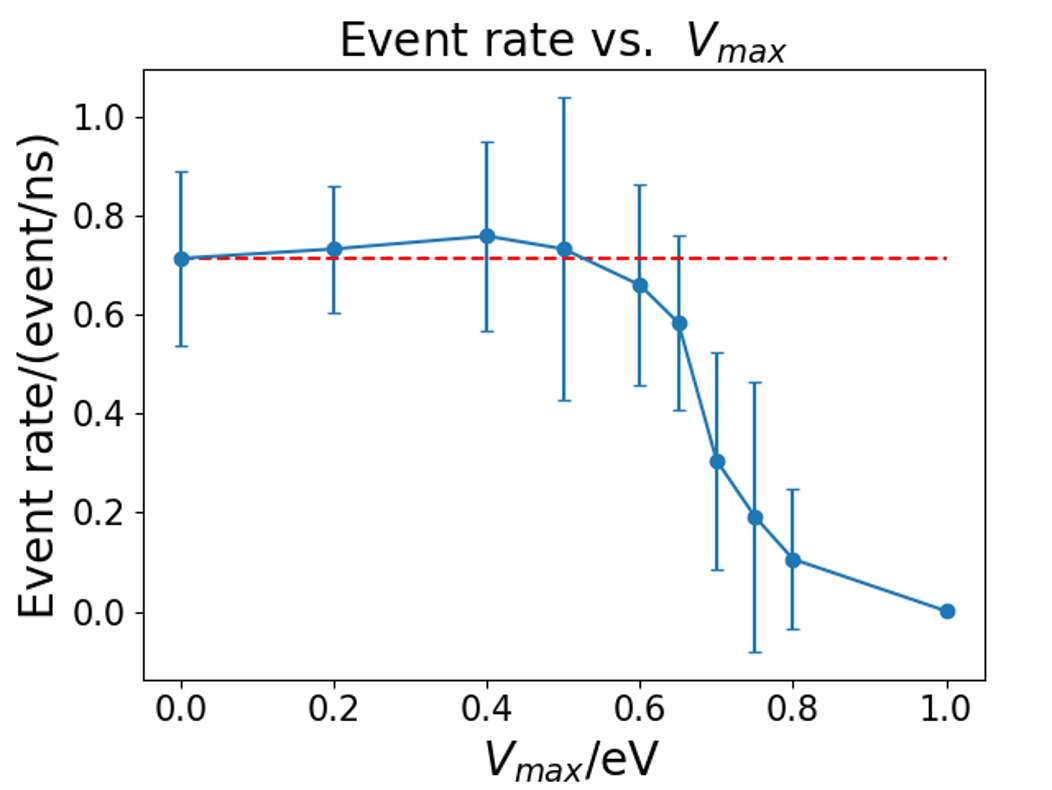
\includegraphics[height=5cm]{event rate.png}
  	\caption{The event rate with different maximum boosts. Each $V_{max}$ has 16 GHD simulations for the time period from 50ns to 125ns}
\end{figure}

The time boost factor ($B_T$) is to measure how much more efficient the HD simulation is than the traditional MD simulation. Usually, we have bigger time boost factors with bigger maximum boost ($V_{max}$). However, the results will be false if $V_{max}$ is too big. We could tell if the result is wrong by calculating the event rate with Eqn. 1.

\begin{equation}
r_{event} = \frac{N_{event}}{t*B_T}
\end{equation}

where $r_{event}$ is the event rate, $N_{event}$ is the number of times that event happens, $t$ is the simulation time and $B_T$ is the time boost factor in this simulation.

As shown in Figure 2, we can tell that the event rates with $V_{max}$ equal or smaller than 0.5eV are consistent with zero $V_{max}$ (regular MD). Hence, we will define the best boost as the biggest boost of which the event rate is the same as the regular MD. In this case, the best boost is $\sim$0.5eV. The reason for rate decreasing is that we will create big artificial barriers and artificial minimums with big $V_{max}$ so that the Ag adatom will be trapped in the artificial minimums and hard to trigger an event.

\section{The stair property}

\subsection{What is the stair property}

\begin{figure}[ht]
	\centering
	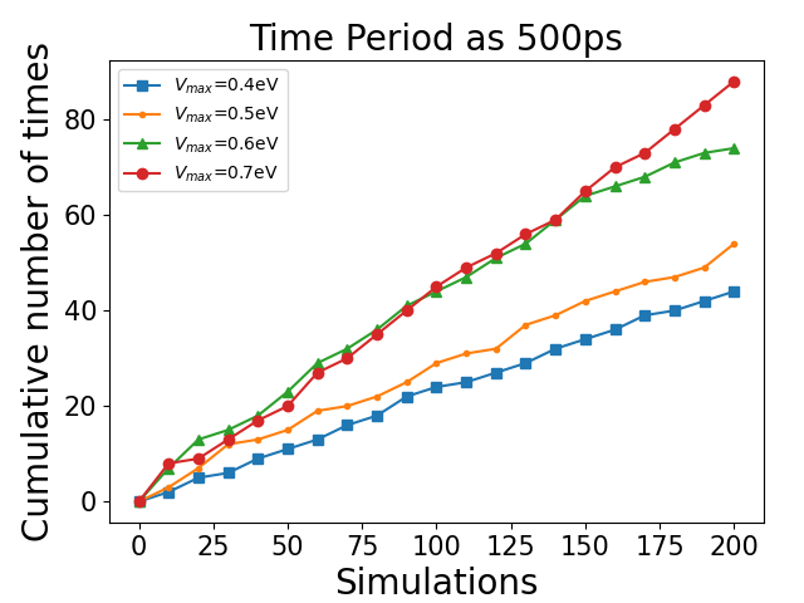
\includegraphics[height=5cm]{500ps.png}
	\caption{The cumulative number of times that events happen in short time period.}
\end{figure}

First, we ran 200 simulations with the time period of 500ps for four $V_{max}$ and count the cumulative number of times that events happen every 10 simulations. The result is shown in Figure 3. It should be noticed that only the appropriate time period will show a result like this. With too short ones, no event will happen with any $V_{max}$. With too long ones, events will happen in every simulation with any $V_{max}$. From Figure 3, we can tell that the cumulative number of times shows a linear relationship with the number of simulation times and the slope should be the probability that events happen with certain time period and $V_{max}$. Furthermore, the gap between 0.5eV and 0.6eV is bigger than others, which implies that the probability might have a sudden change around 0.5eV.

Then, we test a series of $V_{max}$ from 0.30eV to 0.80eV. We simulate 200 times for each $V_{max}$ and count the cumulative number of times that events happen every 10 simulations. The probability that events happen with certain $V_{max}$ is calculated by linear fitting between the cumulative number of times and the simulation times. As shown in Figure 4, the probability-$V_{max}$ plot shows the stair property. Based on the fact that the best boost is $\sim$0.5eV, we can tell that the best boost is the biggest boost on the first level.

\begin{figure}[ht]
	\centering
	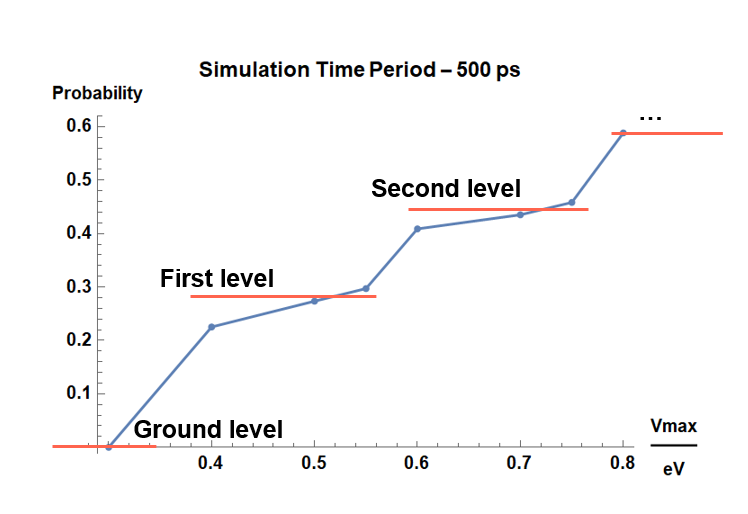
\includegraphics[height=5cm]{stair.png}
	\caption{Stair property between the probability and $V_{max}$}
\end{figure}

\subsection{The stair property holds well with different parameters}

\begin{figure}[ht]
	\centering
	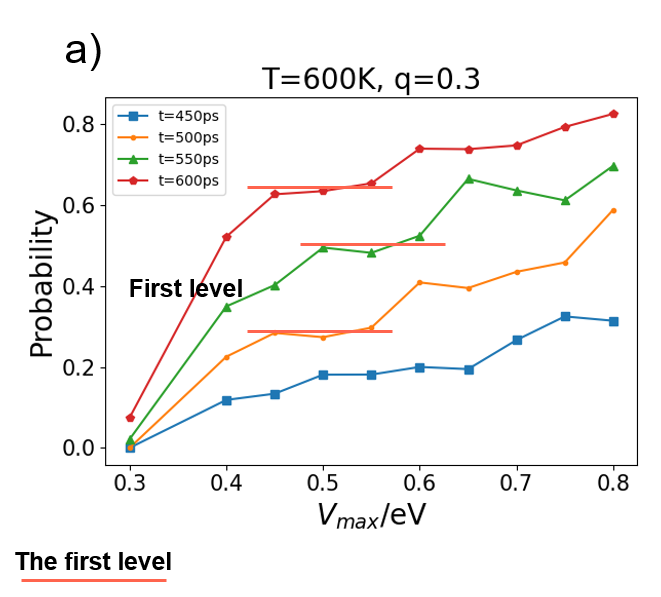
\includegraphics[height=5cm]{different t.png}
	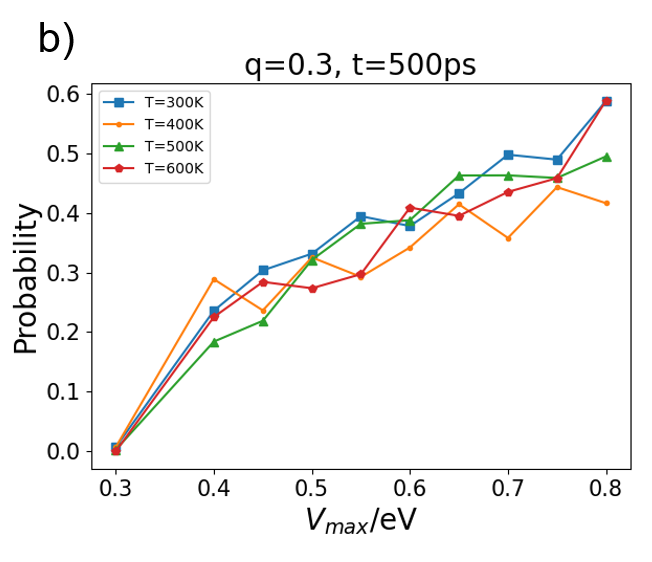
\includegraphics[height=5cm]{different temp.png}
	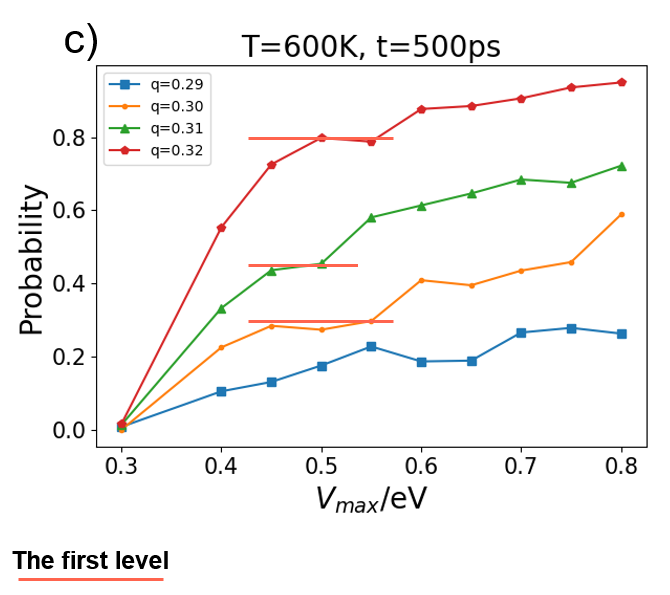
\includegraphics[height=5cm]{different q.png}
	\caption{Stair property between the probability and $V_{max}$. a) Stair property with different time periods. b) Stair property with different temperatures. c) Stair property with different boost threshold.}
\end{figure}

We also run simulations with different time periods, temperatures and boost thresholds. Figure 5a) shows the stair property with different time periods. We can tell that with longer time periods, the probabilities are increasing. All plots exhibit stair property and best boost predictions are 0.55eV or 0.60eV, except the case with 450ps. Hence, 450ps is not a decent time period because the stairs are not obvious due to the small probabilities. The stair property with different temperatures is shown in Figure 5b). The probability seems not to depend on the temperature, although the event rate should be bigger with higher temperature. The reason for this is that the simulation time periods are so short that the different in event rate has not exhibited yet. We can tell all plots exhibit stairs and the best boost predictions is around 0.50eV. Figure 5c) shows the stair property with different boost thresholds. The probability is very sensitive to the boost threshold, even 0.01 difference will lead to an significant change on the plot. The probabilities are increasing with bigger q. This is because the bigger q factor will lead to a bigger boost region. All plots show obvious stairs and the best boost predictions are around 0.50eV except for $q=0.29$. 0.29 is not a decent number for q in this case because of the unobvious stairs. Overall, the stair property will hold with different good parameters, which means we could use it to make the best boost prediction.

\subsection{The stair threshold}

\begin{figure}[ht]
	\centering
	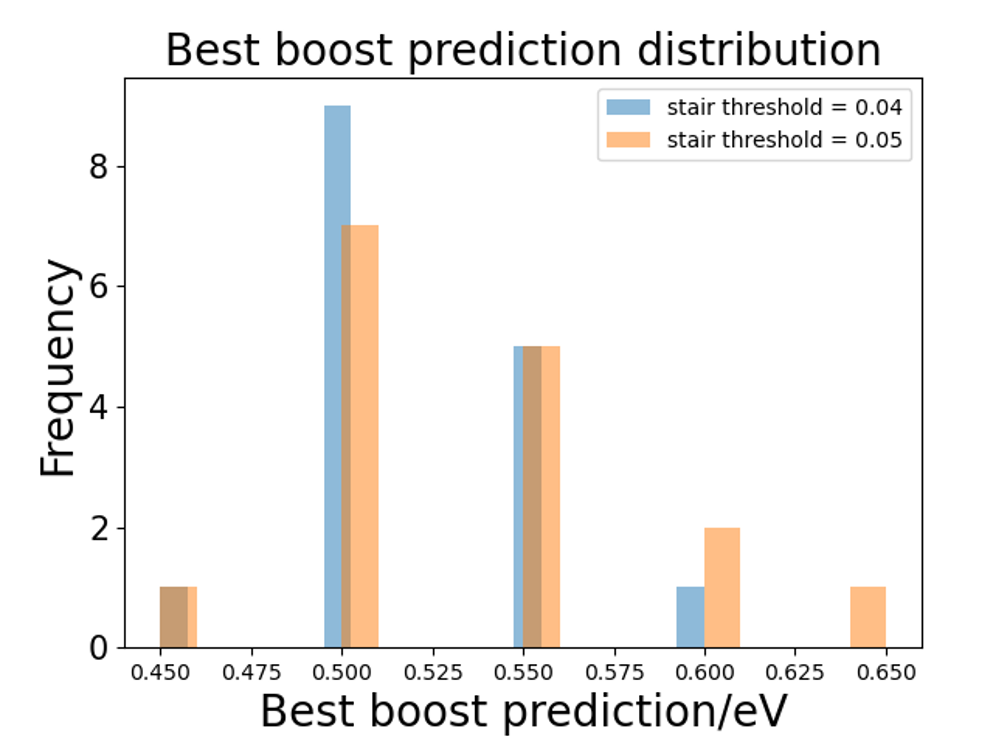
\includegraphics[height=5cm]{stair threshold.png}
	\caption{Comparison between stair thresholds as 0.04 and 0.05}
\end{figure}

We still need to quantitatively define the stair threshold before using the stair property to make predictions. The stair threshold is a number that decides whether the probability is staying on the same stair or climbing to the next stair. If the probability difference from the last $V_{max}$ is bigger than the stair threshold, we will say it is climbing to the next stair. Otherwires, it is staying on the same stair with the last $V_{max}$. Figure 6 is the comparison between 0.04 and 0.05. We used four sets of parameters: 1. t=500ps, q=0.30; 2. t=550ps, q=0.30; 3. t=600ps, q=0.31; 4. t=500ps, q=0.31. We made four predictions for each set of parameters. The predictions show good consistency. The stair threshold as 0.04 gives more compact predictions so that it is better than 0.05. Hence, we will use the stair property to make best boost prediction and set the stair threshold as 0.04.

\section{Python + LAMMPS}

Since LAMMPS cannot adjust the parameters by itself, we also need Python to realize the AHDM algorithm. The workflow is shown as following:

1. Input: a series of time periods, a series of $V_{max}$ and iterations for each $V_{max}$

2. Write LAMMPS input files based on the inputs. Each iteration needs a special Langevin seed.

3. Run GHD simulations (in parallel on multi-processors if possible)

4. For each time period, count the cumulative number of times that events happen every ten iterations for each $V_{max}$

5. For each time period, linear fit the cumulative number of times that events happen with the simulation times for each $V_{max}$. The slopes are the probabilites that events happen.

6. For each time period, decide if the probability-$V_{max}$ plot is good. For a good plot, the following requirements should be fulfilled: a) The probabilities of the smallest two $V_{max}$ should be bigger than 0.04. This is to make sure we have the ground level. b) The probability of the biggest $V_{max}$ should be bigger than 0.4. This is to make sure we have obvious stairs. c) The probabilities of the biggest two $V_{max}$ should be smaller than 0.95. This is to get rid of the time periods that are too long. With too long time period, we will not be able to where the first level ends.

7. For each good time period, calculate the probability difference from the beginning. We have made sure the plots will start from the ground level in step 6. Hence, if the difference is smaller than 0.04, we will say it is still on the ground level. When the difference is bigger than 0.04, we will say it starts to climbing to the first level.

8. Keep calculating the difference. If the difference is bigger than 0.04, we will say it is still climbing to the first level. When the difference is smaller than 0.04, we will say that it is on the first level.

9. Keep calculating the difference. If the difference is smaller than 0.04, we will say it is still on the first level. When the difference is bigger than 0.04, we will say it starts to climb to the second level. Stop calculating the difference.

10. For each good time period, choose the biggest $V_{max}$ on the first level as the prediction of the best boost.

11. Collect all the predictions from the good time periods. Choose the most predicted $V_{max}$ as the result.

\section{Conclusion}

We discover the stair property in GHD between the probability and the boost, which could be used to predict the best boost. The best boost is the biggest boost of which the event rate keeps consistant with the traditional MD. We find out the best boost is the biggest boost on the first level and we develop the AHDM algorithm to automatically predict the best boost by testing a series of $V_{max}$ for a series of time periods and choosing the most predicted best boost as the result.

\bibliography{ref}
\end{document}